\documentclass[journal,10pt]{IEEEtran}
\usepackage{amsmath,amssymb,amsthm}
\usepackage{booktabs,array,graphicx}
\usepackage{cite}
\usepackage{url}
\usepackage{needspace}
\usepackage[hidelinks]{hyperref}
\newcommand{\E}{\mathbb{E}}
\newcommand{\R}{\mathbb{R}}
\newcommand{\HF}{\mathrm{H}}
\newcommand{\LF}{\mathrm{L}}
\newcommand{\Var}{\operatorname{Var}}
\newcommand{\Cov}{\operatorname{Cov}}
\newcommand{\pending}[1]{\par\noindent\textit{Pending: #1}\par}
\newtheorem{proposition}{Proposition}
\newtheorem{assumption}{Assumption}
\title{Supplementary Material: Information-Stratified Policy Optimization}
\author{Research working draft}
\markboth{ISPO Supplementary Working Draft, October 11, 2026}{ISPO Supplementary Material}
\begin{document}
\maketitle
\noindent This supplement preserves detailed evaluator, gradient and recording evidence accompanying the research working draft. Each result has a source-bound repository receipt; incomplete study questions remain labeled in the main paper.
\section{Original-Task Multifidelity Baseline}
The complete original Hopper-v3 study uses twenty registered training seeds per method with the source-explicit state and evaluation corrections described in the repository. Low- and high-fidelity coupling and the native guarded optimizer semantics are retained. Every run reaches its full registered HF horizon. Terminal-only import verifies state/API traces, actual sample counts, checkpoints, initial-policy identities and full process costs before the aggregate is computed. Separate final evaluation is kept distinct from the last periodic evaluation.

Figure~\ref{fig:original-mfpg} compares the full curves with the published reference~\cite{liu2025mfpg}. The reproduction supports the original MFPG improvement over its HF-only counterpart. Published and reproduced means are descriptive comparisons; the plotted intervals are pointwise mean confidence bands. This experiment validates the baseline implementation on its original task. The shared-design comparison with ISPO remains part of the main experimental program.

\begin{figure*}[t]
\centering
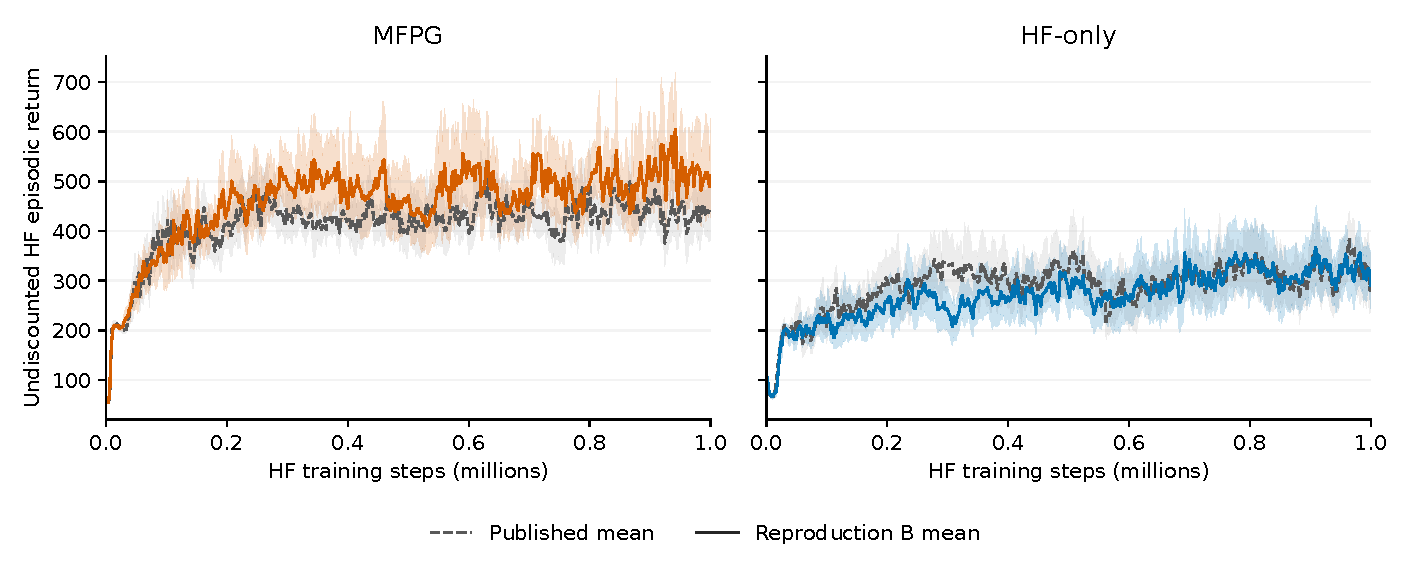
\includegraphics[width=\textwidth]{figures/mfpg_original_cohort.pdf}
\caption{Full original-task Hopper-v3 curves with LF gravity factor 0.8. Each method retains all twenty seeds. Solid curves show source-explicit reproduction B; dashed curves show published means. Shading denotes pointwise 95\% seed-bootstrap mean intervals. Native state restoration and evaluation isolation are recorded as implementation corrections, with their original failures and costs retained.}
\label{fig:original-mfpg}
\end{figure*}
\section{Physical and Estimator Verification}
The initial coupled Boussinesq cavity evaluator has passed its declared physical and derivative verification gate. Coarse and fine evaluations close their discrete residual and mass/heat balances; removing buoyancy changes the coupled residual, and both continuous design sensitivities agree with directional finite differences at two step sizes. The field interface evaluates the actual fine-grid residual on an interpolated coarse state without a fine-grid solve. A third grid supplies a sensitivity check, while lid reversal and heat-band relocation produce distinct physical responses. Failed forward attempts remain in the immutable run record.

The gate identifies a reusable reference evaluator for the first mechanism study, with a pinned residual/adjoint dependency and verified adapter identity. Its scope is the declared cavity configuration, selected design perturbations, and the recorded grids; the mesh check is a sensitivity observation rather than a continuum error certificate. The source receipt is linked by run identity in the repository completion audit, with raw plus/minus evaluations independently recomputed before acceptance.
\subsubsection{Mixed-cooling information interfaces}
The Shinaide playground has a source-bound liquid steady evaluator and a fan-assisted zonal air model that retains the saved server identities, airflows and heat budgets. Initial interface checks preserve the authored equipment and containment geometry. Independent state reconstruction verifies the coupled mass and enthalpy equations, per-server heat transport and room heat closure; two-step directional checks support a joint perturbation of the air-conditioning controls. The zones and passage laws are declared low-fidelity assumptions.

A derived six-ACU OPEN reference satisfies the registered synthetic thermal, capacity, hydraulic and airflow requirements in nominal operation and every single-unit outage. Both physical branches use the same saved project, and the failed unit has closed ports and zero cooling duty. Independent reconstruction from the accepted states agrees with the device electricity account and resulting objective. This provides a feasible reference for the flagship design task. The equal outage responses follow the current model's common mixing nodes and interchangeable equipment; location-dependent outage behavior will be evaluated by the corresponding room CFD checks.

The liquid evaluator uses the packed physical parameters and a nominal pump-affinity law. Changing the pump speed in the project, recompiling it, and resolving the full steady system at four registered perturbations verifies implicit sensitivities of hydraulic work and a fixed chip temperature. The linearization includes the solved flow and temperature response and the native conserved-storage constraints. Independent matrix and state reconstruction agrees with the two-step finite differences. Hydraulic work is distinguished from electrical input, which requires an explicitly declared efficiency.

A shared plant model accounts for the air and liquid loads with one IT denominator and one primary cooling plant. Its coilwise temperature constraints, branch mixing, fan power, and secondary pumping were checked against the same-source fields and independent energy arithmetic. The current equipment parameters and heat budgets are mock inputs. Fixed server airflow and prescribed steady cold-plate heat partition remain part of this benchmark definition. A tie between active branches with different sensitivities makes the hard plant rule nonsmooth; an automatic-differentiation subgradient is then not identified as a unique ordinary derivative.

At a separately saved operating point with distinct active branches and interior flows, the compound liquid--air oracle returns a source-consistent PUE and nine-control gradient. Independent reconstruction separates equipment algebra from the solved air and liquid responses. One predeclared joint direction agrees with fresh two-step finite differences, with unchanged active branches. This is an energy-only directional check, not nine independent directions or the full constrained reward; the changed nominal PUE is not an optimization gain. Comparison methods must receive the same known-algebra treatment so that it is not credited as a physical-adjoint benefit.

The high-fidelity fan export preserves server identities, paired faces, airflow and residual air heat from the same liquid evaluation. Its new paired-flow air-conditioning mode explicitly matches the network assumption; legacy pressure-return boundaries do not impose that constraint. A conservative fan condition includes convective and diffusive transport. Field and library-loading checks pass, while actual mesh startup, component flux compatibility and room heat closure await high-fidelity acceptance.

\subsubsection{Aerodynamic derivative interface}
For the declared finite-trailing-edge airfoil, a discrete adjoint was constructed from the complete native residual, including cell variables and internal and far-field face fluxes. An independent audit reconstructs its transpose equation and compares a full-rank set of 17 parameter directions with 68 actual forward evaluations at two step sizes. The maximum relative discrepancy is below $3.2\times10^{-4}$ on these directions. A separate matched two-grid audit reconstructs all 17 sensitivities from the original signed parameter-operator outputs and accepted transpose solutions. The component changes satisfy the registered grid-sensitivity gate; this is a sensitivity observation rather than a continuum error certificate. These checks qualify gradient information at the sampled baseline. Broader design conditions and aerodynamic post-training require separate evidence.

An additional gate exercises the established DAFoam interface on its pinned official NACA0012 problem~\cite{he2020dafoam}. This is a different Reynolds number and drag objective from the native lift case above. Its original symmetry boundaries are retained, with an applicable two-dimensional mesh diagnostic and the solver's native checks. Independent reconstruction from the saved adjoint arrays verifies the normalized transpose residual, and the drag sensitivity to angle of attack agrees with two-step finite differences. The gate establishes that specific primal/adjoint route; it does not establish matching between the two aerodynamic problems, full shape sensitivities or training benefit.

The supported CST16 benchmark connects the reference-preserving surface map to IDWarp and the native flow and force components. Fixed span pairing and farfield are included in both tangent and reverse mappings. Full sixteen-direction central differences at two registered step sizes verify the raw drag and lift derivatives at the declared coarse-grid center. The complete residual transpose is independently reconstructed from saved arrays. A wall-distance registration bridge retains the native distance algorithm and its geometry update, closing a shape-derivative path that had been frozen in the initial implementation. The repaired forward values match the original cold-forward values. All original failed gates and costs remain in the repository evidence. These results qualify the local force-gradient vector; refined-grid, broader-domain and discontinuous hard-reward derivatives remain separate questions.

\subsubsection{External-physics language-policy bridge}
The stochastic numerical interface was executed with text checkpoints of approximately 4.2 and 26.9 billion parameters. Every proposal was preserved as a schema-valid engineering document and evaluated by the same coupled finite-volume target. In the interface gates, scalar reward gradients and parameter sensitivities from the external target both reached the trainable language adapters. The small checkpoint completed two updates from eight target evaluations; the large checkpoint completed one update from two evaluations. The corresponding short, 90-token interface used approximately 8.7 and 52.3 GiB peak allocated GPU memory, respectively, on a single device. These gates establish the intended gradient route and a measured resource envelope for this restricted interface; they do not establish training benefits or memory for long layout sequences.

\subsubsection{Common SFT start and online execution}
Sixteen legal heuristic designs from four training tasks supplied a common supervised start, without high-fidelity optimization labels. The executed task family varies geometry, material coefficients and heating-boundary width; its physical coordinates and sensitivities were independently checked. The complete language adapter and numerical head were frozen as the reference. High-fidelity RLOO, scalar augmented correction and conditional LAX then each completed four online updates from that same start, with genuine proposal documents and fresh physical calls. Sparse target purchases included a retained zero-target batch. Initial and final held-out checks were excluded from optimization and checkpoint selection. These pilots establish the executed feedback and recording contract; their single seed and small evaluation count do not supply the main cost--quality or generalization result.

\subsubsection{Objective-aware residual mechanism}
A preregistered set of 60 designs was evaluated at both cavity fidelities, with all attempted outcomes and costs retained. On its 12 predeclared diagnostic anchors, the adjoint-weighted correction was constructed using only the interpolated coarse state and the exact target operator, without a target forward solve or use of target fields. The target scalar was read only after prediction persistence for independent post-validation. Table~\ref{tab:goal-correction} separates the correction's numerical effect from its acquisition cost.
\begin{table}[t]
\centering
\caption{Bounded goal-correction mechanism on 12 predeclared cavity designs. Errors concern the common thermal objective, not field error.}
\label{tab:goal-correction}
\begin{tabular}{lr}
\toprule
Quantity & Measured value \\
\midrule
Mean absolute coarse-goal error & $2.5171\times10^{-3}$ \\
Mean error after target-grid mapping & $2.1311\times10^{-3}$ \\
Mean error after adjoint correction & $2.0240\times10^{-4}$ \\
Largest transpose relative residual & $2.25\times10^{-13}$ \\
Largest directional FD relative error & $2.05\times10^{-8}$ \\
Correction work, 12 designs (s) & $5.76$ \\
Additional one-time setup (s) & $4.63$ \\
\bottomrule
\end{tabular}
\end{table}
The raw or fixed-block-scaled residual norms did not positively rank the original thermal-goal error on these anchors. The absolute predicted total goal discrepancy from the adjoint construction had positive rank association with that same error. This distinction motivates the objective-aware interface: the useful signal estimates the quantity being optimized rather than assuming that an aggregate equation norm is sufficient. No total-budget learning gain is inferred from the correction table; mapping, Jacobian, transpose-solve and setup charges remain in the acquisition ledger.

A companion channel entry changes the physical layout through inlet-opening and heated-baffle choices. Two representative structures passed primal, flux and parameter-sensitivity checks, while independent parsed-polyhedron tests verified the solids and mesh closure. Its lifting uses convex supports that avoid the obstacle and retains the pinned outlet-pressure reference. On two predeclared anchors, adjoint-weighted goal correction improved postvalidated output estimates without a target forward solve during prediction. The mapped fields retain their mass and heat defects as residual information; they are not treated as target-converged fields. Corrected design derivatives and the four-structure learning study require separate evidence.

\subsubsection{Fixed-policy estimator and instrument-cost checks}
The paired response table also supplies an exactly computable gradient for a categorical policy over its physical designs. The reference estimator diagnostic uses independent prior calibration, ten calibration seeds and fixed proposal concentrations. It handles the analytic actuator term exactly for all baselines. Cached table sampling is labeled as a response-table diagnostic, while hypothetical call budgets use measured warm-forward timings and disclose original dataset and calibration charges. On the initial instrument, the coarse-grid forward call was slightly more expensive than the fine-grid call; forcing a multifidelity arm consequently provided no economic benefit. Including the target-only arm selects it under that measured cost structure. Independent exact-Jacobian solver profiling is therefore part of the implementation audit before the main learning experiment; neither a mesh label nor high reward correlation substitutes for a measured cheap-interface cost.

\subsubsection{Measured language-parameter gradient mechanism}
The fixed complete-SFT small language policy generated 24 independent four-design groups across four physical training contexts. Eight past groups calibrated coefficients; sixteen fresh groups supplied analysis without recalibration. All 96 designs received new cheap-gradient and target evaluations. Complete trainable-parameter vectors were stored, with no random projection or optimizer update. The joint-score RLOO construction in the main paper's group value/path construction was independently recomputed; exact acquisition-mask enumeration verified its conditional moments.

Averaged within-context target-gradient trace was $0.9498$. Past-calibrated LAX traces at purchase probabilities $0.1$, $0.5$ and $1$ were $0.3371$, $0.1575$ and $0.1133$; scalar augmented correction gave $1.1519$, $0.9723$ and $0.9498$. These descriptive fixed-policy moments use four fresh groups per context. Fixed-unit LAX at $q=0.1$ instead gave $6.3307$, exposing the role of predictable calibration. At the same value coefficient the methods have identical conditional purchase noise; the cheap path/score control changes proposal-group variability. Separate FP32 basis assembly and native BF16 backward differed by at most $0.00587$ in relative norm.

Collection purchased every pair and consumed $349$~s of full process wall time. Expected warm physical-call charges are not achieved online savings: sixteen target-only groups cost $113$~s, versus $68.5$~s for the $q=0.1$ cheap-gradient/purchase model before calibration. Past calibration physical calls add $99.7$~s; their complete model/recording cost is not isolated from the collection meter. The variance mechanism thus motivates a moving-policy, fully charged comparison rather than establishing training or short-budget efficiency.

The task-normalized goal interface passed prediction, transpose, directional and optional-failure checks. Its auxiliary value is separated from the original cheap derivative. A four-update residual-value LAX pilot executed this route, with sixteen cheap-gradient and fourteen target calls. A separate four-option channel policy executed genuine inlet/baffle choices and the cheap-gradient route. Its initial/final checks concern the same problem; neither pilot establishes generalization or the main comparison.


\bibliographystyle{IEEEtran}
\bibliography{references}
\end{document}
